\documentclass[10pt,aspectratio=169]{beamer}

% ---------- Theme ----------
\usetheme{metropolis}
\metroset{progressbar=frametitle}

\usepackage[T1]{fontenc}
\usepackage[utf8]{inputenc}
\usepackage{listings}
\usepackage{xcolor}
\usepackage{tikz}
\usepackage{hyperref}

% --- Logos on the title slide (top right) ---
% 'assets/Logo MEVIS 14_mevis_rgb.png' and 'assets/UHB_Logo_Englisch_Web_RGB.png'
% live next to this .tex file.
\addtobeamertemplate{title page}{%
  \begin{tikzpicture}[remember picture,overlay]
    \node[anchor=north east,inner sep=0pt,xshift=-0.5cm,yshift=-0.4cm]
      at (current page.north east)
      {
\includegraphics[height=0.9cm]{assets/Logo MEVIS 14_mevis_rgb.png}};
    \node[anchor=north east,inner sep=0pt,xshift=-0.5cm,yshift=-1.7cm]
      at (current page.north east)
      {
\includegraphics[height=0.8cm]{assets/UHB_Logo_Englisch_Web_RGB.png}};
  \end{tikzpicture}%
}{}

% ---------- Colors for code ----------
\definecolor{codebg}{RGB}{245,245,245}
\definecolor{codekw}{RGB}{0,102,204}
\definecolor{codestr}{RGB}{163,21,21}
\definecolor{codecom}{RGB}{0,128,0}
\definecolor{codenum}{RGB}{120,120,120}

% ---------- Listings setup for Python ----------
\lstdefinestyle{pythonstyle}{
  language=Python,
  backgroundcolor=\color{codebg},
  basicstyle=\ttfamily\scriptsize,
  keywordstyle=\color{codekw}\bfseries,
  stringstyle=\color{codestr},
  commentstyle=\color{codecom}\itshape,
  numberstyle=\tiny\color{codenum},
  numbers=left,
  numbersep=6pt,
  showstringspaces=false,
  breaklines=true,
  breakatwhitespace=true,
  frame=single,
  rulecolor=\color{black!20},
  framexleftmargin=4pt,
  framexrightmargin=2pt,
  xleftmargin=12pt,
  tabsize=2,
  columns=fullflexible,
  keepspaces=true,
  morekeywords={as,with,True,False,None,self,lambda}
}
\lstset{style=pythonstyle}
\renewcommand{\section}[2][]{}
\usepackage{courier}

% ---------- Title ----------
\title{Brain Tumor Segmentation using U-Net}
\subtitle{A walk-through of the Python implementation (BraTS 2020)}
\author{Course material presented by Horst Hahn, based on the ipynb on \href{https://www.kaggle.com/code/zeeshanlatif/brain-tumor-segmentation-using-u-net}{kaggle.com by Zeeshan Latif}}
\date{\today}

\begin{document}

\begin{frame}
  \titlepage
\end{frame}

% =====================================================================
\section{Overview}

\begin{frame}{What this notebook does}
  \begin{itemize}
    \item Input: brain MRI scans from the \textbf{BraTS 2020} dataset. Each patient
          has four modalities (T1, T1ce, T2, FLAIR) plus an expert segmentation mask.
    \item Goal: predict, for every pixel of every axial slice, which tumor region it belongs to.
    \item The model is a \textbf{2D U-Net} that takes two channels (FLAIR + T1ce) and outputs
          a 4-class probability map.
  \end{itemize}
  \vspace{0.4em}
  \begin{center}
  \begin{tabular}{cll}
    \textbf{Label} & \textbf{Class} & \textbf{Meaning}\\\hline
    0 & NOT tumor       & healthy tissue / background\\
    1 & Necrotic / Core & non-enhancing tumor core\\
    2 & Edema           & swelling around the tumor\\
    3 & Enhancing       & enhancing tumor (BraTS label 4 $\to$ 3)\\
  \end{tabular}
  \end{center}
\end{frame}

\begin{frame}{The pipeline at a glance}
  \begin{enumerate}
    \item \textbf{Download \& unzip} the dataset (Kaggle CLI).
    \item \textbf{Explore} the modalities and masks (slices, montages, per-class views).
    \item \textbf{Preprocess}: scale to $[0,1]$, resize slices to $128\times128$.
    \item \textbf{Split} cases into train / validation / test.
    \item \textbf{Stream} data to the network with a custom \texttt{DataGenerator}.
    \item \textbf{Define} the U-Net, the Dice loss, and evaluation metrics.
    \item \textbf{Train}, checkpoint the best weights, and save the model.
    \item \textbf{Predict} and visualize segmentations on test patients.
  \end{enumerate}
\end{frame}

% =====================================================================
\section{Setup and imports}

\begin{frame}[fragile]{Getting the data and the libraries}
\begin{columns}[T,onlytextwidth]
\begin{column}{0.42\textwidth}
\small
The leading \texttt{!} runs a \emph{shell} command from inside the notebook. We install the
Kaggle CLI, drop in the API token, and download + unzip the dataset.\\[0.4em]
The \texttt{unzip} pattern \texttt{BraTS20\_Training\_0[0-9][0-9]} only extracts cases
000--099 (plus 100), keeping the download small.\\[0.4em]
The imports cover arrays (\texttt{numpy}), images (\texttt{cv2}, \texttt{nibabel} for
\texttt{.nii} files), plotting (\texttt{matplotlib}), and the deep-learning stack
(\texttt{keras} / \texttt{tensorflow}).
\end{column}
\begin{column}{0.56\textwidth}
\begin{lstlisting}[firstnumber=last]
!pip install kaggle
!kaggle datasets download awsaf49/brats20-...
!unzip brats20-...zip \
  'BraTS2020_TrainingData/.../BraTS20_Training_0[0-9][0-9]/*'

import os, cv2, glob, random
import numpy as np
import pandas as pd
import nibabel as nib              # reads .nii MRI volumes
import matplotlib.pyplot as plt
from skimage.util import montage
from skimage.transform import rotate
import keras, tensorflow as tf
import keras.backend as K
from sklearn.preprocessing import MinMaxScaler
from sklearn.model_selection import train_test_split
from tensorflow.keras.layers import *
from tensorflow.keras.models import *
\end{lstlisting}
\end{column}
\end{columns}
\end{frame}

% =====================================================================
\section{File paths}

\begin{frame}[fragile]{One helper for every file path}
\begin{columns}[T,onlytextwidth]
\begin{column}{0.42\textwidth}
\small
Every scan lives at a predictable path. Instead of rebuilding that string by hand in a dozen
places, the notebook centralizes it in \textbf{one} helper.\\[0.4em]
\texttt{caseDir} formats the folder name; \texttt{imgPath} appends the modality and the
\texttt{.nii} extension.\\[0.4em]
A case can be given as a number (\texttt{55}) or a string (\texttt{"055"}) -- \texttt{int(case)}
normalizes both before formatting.
\end{column}
\begin{column}{0.56\textwidth}
\begin{lstlisting}[firstnumber=last]
TRAIN_DATASET_PATH = \
  "BraTS2020_TrainingData/MICCAI_BraTS2020_TrainingData/"

# Build the path to any modality of any case number.
def caseDir(case):
    return TRAIN_DATASET_PATH + \
        f"BraTS20_Training_{int(case):03d}/"

def imgPath(case, mriType):
    return f"{caseDir(case)}" \
        f"BraTS20_Training_{int(case):03d}_{mriType}.nii"

# e.g. imgPath(55, 'flair') ->
#   ".../BraTS20_Training_055/BraTS20_Training_055_flair.nii"
\end{lstlisting}
\end{column}
\end{columns}
\end{frame}

\begin{frame}[fragile]{Python syntax: f-strings and format specs}
\begin{columns}[T,onlytextwidth]
\begin{column}{0.42\textwidth}
\small
\textbf{f-strings} (the \texttt{f"..."} prefix) let you embed expressions directly inside a string
using \texttt{\{\,\}}.\\[0.4em]
\textbf{The \texttt{:03d} format spec} means: format as an integer (\texttt{d}), pad with zeros
(\texttt{0}) to a width of 3. So \texttt{7} becomes \texttt{"007"}.\\[0.4em]
This is why the case number always appears as three digits, matching the folder names on disk.\\[0.4em]
\textbf{Why \texttt{int(case)}?} A string like \texttt{"55"} has no numeric format, so we convert
first; \texttt{int("055")} is also \texttt{55}, so both forms collapse to the same path.
\end{column}
\begin{column}{0.56\textwidth}
\begin{lstlisting}[stepnumber=0]
case = 7
f"{case:03d}"          # -> "007"
f"{int('55'):03d}"     # -> "055"

# An f-string evaluates whatever is inside {...}:
name = "flair"
f"...{name}.nii"       # -> "...flair.nii"

# Equivalent old-style formatting:
"{:03d}".format(case)  # -> "007"
\end{lstlisting}
\end{column}
\end{columns}
\end{frame}

% =====================================================================
\section{Loading and scaling}

\begin{frame}[fragile]{Loading a volume and scaling it to [0, 1]}
\begin{columns}[T,onlytextwidth]
\begin{column}{0.42\textwidth}
\small
MRI intensities are arbitrary (a FLAIR scan can peak near 1800). Neural networks train better on
inputs in a fixed range, so we rescale each volume to $[0,1]$ with \texttt{MinMaxScaler}.\\[0.4em]
\texttt{nib.load(...).get\_fdata()} returns the 3D volume as a NumPy array of shape
$(240, 240, 155)$.\\[0.4em]
The mask (\texttt{seg}) is \emph{not} scaled -- its values are class labels, not intensities.\\[0.4em]
\texttt{load\_scaled} wraps this so the four modalities are loaded with one call each.
\end{column}
\begin{column}{0.56\textwidth}
\begin{lstlisting}[firstnumber=last]
scaler = MinMaxScaler()

def load_scaled(case, mriType):
    img = nib.load(imgPath(case, mriType)).get_fdata()
    return scaler.fit_transform(
        img.reshape(-1, img.shape[-1])
    ).reshape(img.shape)

test_image_t1    = load_scaled(ex_case, 't1')
test_image_t1ce  = load_scaled(ex_case, 't1ce')
test_image_flair = load_scaled(ex_case, 'flair')
test_image_seg   = nib.load(
    imgPath(ex_case, 'seg')).get_fdata()   # labels: no scaling
\end{lstlisting}
\end{column}
\end{columns}
\end{frame}

\begin{frame}[fragile]{Python syntax: the reshape / scale / reshape trick}
\begin{columns}[T,onlytextwidth]
\begin{column}{0.42\textwidth}
\small
\texttt{MinMaxScaler} works on 2D data (samples $\times$ features). Our image is 3D, so we
flatten, scale, then restore the shape.\\[0.4em]
\textbf{\texttt{reshape(-1, n)}} -- the \texttt{-1} means ``figure out this dimension
automatically''. With \texttt{n = img.shape[-1]} (= 155 slices) we get a 2D array of
$(240\!\cdot\!240,\ 155)$.\\[0.4em]
\texttt{fit\_transform} then min-max scales it, and the final \texttt{reshape(img.shape)} puts it
back to $(240, 240, 155)$.\\[0.4em]
Net effect: every voxel ends up in $[0,1]$, shape unchanged.
\end{column}
\begin{column}{0.56\textwidth}
\begin{lstlisting}[stepnumber=0]
img.shape            # (240, 240, 155)

# 1) flatten to 2D: rows = pixels, cols = slices
flat = img.reshape(-1, img.shape[-1])
flat.shape           # (57600, 155)

# 2) min-max scale each column into [0, 1]
scaled = scaler.fit_transform(flat)

# 3) restore the original 3D shape
out = scaled.reshape(img.shape)
out.shape            # (240, 240, 155)
\end{lstlisting}
\end{column}
\end{columns}
\end{frame}

% =====================================================================
\section{Exploring the data}

\begin{frame}[fragile]{Three anatomical views of one slice}
\begin{columns}[T,onlytextwidth]
\begin{column}{0.42\textwidth}
\small
A 3D volume can be cut along three axes. By indexing different axes of the same array we get the
transverse, frontal, and sagittal views.\\[0.4em]
\texttt{rotate(..., 90, resize=True)} turns the slice upright and resizes the canvas so nothing is
clipped.\\[0.4em]
\textbf{Reading the slicing:} \texttt{vol[:,:,k]} fixes the 3rd axis (one axial slice),
\texttt{vol[:,k,:]} fixes the 2nd, \texttt{vol[k,:,:]} fixes the 1st.
\end{column}
\begin{column}{0.56\textwidth}
\begin{lstlisting}[firstnumber=last]
# Transverse (axial)
plt.imshow(test_image_t1ce[:, :, slice], cmap='gray')

# Frontal (coronal)
plt.imshow(rotate(test_image_t1ce[:, ex_tumor_pos[1], :],
                  90, resize=True), cmap='gray')

# Sagittal
plt.imshow(rotate(test_image_t1ce[ex_tumor_pos[2], :, :],
                  90, resize=True), cmap='gray')
\end{lstlisting}
\end{column}
\end{columns}
\end{frame}

\begin{frame}[fragile]{Montage: all slices on one canvas}
\begin{columns}[T,onlytextwidth]
\begin{column}{0.42\textwidth}
\small
\texttt{montage} tiles every slice of a volume into a single 2D image -- handy to scan a whole
brain at a glance.\\[0.4em]
The slicing \texttt{[50:-50,\,:,\,:]} drops the first and last 50 slices, which are mostly empty,
so the montage shows only the informative middle.\\[0.4em]
The trailing semicolon in a notebook just suppresses the text output of the last expression.
\end{column}
\begin{column}{0.56\textwidth}
\begin{lstlisting}[firstnumber=last]
# Whole volume tiled into one image
plt.imshow(rotate(montage(test_image_t1ce[:, :, :]),
                  90, resize=True), cmap='gray')

# Skip empty end-slices -> just the middle
plt.imshow(rotate(montage(test_image_t1ce[50:-50, :, :]),
                  90, resize=True), cmap='gray')
\end{lstlisting}
\end{column}
\end{columns}
\end{frame}

% =====================================================================
\section{Splitting the dataset}

\begin{frame}[fragile]{Train / validation / test split}
\begin{columns}[T,onlytextwidth]
\begin{column}{0.42\textwidth}
\small
\texttt{os.scandir} lists the case folders; \texttt{os.path.basename} turns each full path into just
the case id (e.g. \texttt{BraTS20\_Training\_017}).\\[0.4em]
We split \textbf{twice}: first peel off 20\% for validation, then split the remainder into train
and test. The result is roughly 68\% / 12\% / 20\%.\\[0.4em]
Splitting by \emph{patient id} (not by slice) is important -- it prevents slices of the same brain
leaking across train and test.
\end{column}
\begin{column}{0.56\textwidth}
\begin{lstlisting}[firstnumber=last]
train_and_val_directories = [
    f.path for f in os.scandir(TRAIN_DATASET_PATH)
    if f.is_dir()]

def pathListIntoIds(dirList):
    return [os.path.basename(p) for p in dirList]

ids = pathListIntoIds(train_and_val_directories)

train_test_ids, val_ids = train_test_split(
    ids, test_size=0.2)
train_ids, test_ids = train_test_split(
    train_test_ids, test_size=0.15)
\end{lstlisting}
\end{column}
\end{columns}
\end{frame}

% =====================================================================
\section{The data generator}

\begin{frame}{Why a data generator?}
  \begin{itemize}
    \item The full dataset is far too large to hold in memory at once.
    \item A \texttt{keras.utils.Sequence} streams data \textbf{batch by batch}: Keras asks for batch
          $i$, the generator loads exactly those volumes, hands them over, and frees them.
    \item For each case it keeps \texttt{VOLUME\_SLICES = 100} slices, starting at slice
          \texttt{VOLUME\_START\_AT = 22} (skipping mostly-empty end slices).
    \item Each slice is resized to $128\times128$ and stacked into two input channels
          (\textbf{FLAIR} and \textbf{T1ce}).
  \end{itemize}
  \vspace{0.4em}
  A \texttt{Sequence} subclass must implement three methods: \texttt{\_\_len\_\_} (number of
  batches), \texttt{\_\_getitem\_\_} (build batch $i$), and \texttt{on\_epoch\_end} (reshuffle).
\end{frame}

\begin{frame}[fragile]{\texttt{DataGenerator} (1/2): the skeleton}
\begin{columns}[T,onlytextwidth]
\begin{column}{0.42\textwidth}
\small
\texttt{\_\_len\_\_} tells Keras how many batches make one epoch.\\[0.4em]
\texttt{\_\_getitem\_\_} is called with a batch index; it slices out the ids for that batch and
delegates to the data-loading routine.\\[0.4em]
\texttt{on\_epoch\_end} reshuffles the order after every epoch (only if \texttt{shuffle=True}), so
the network never sees batches in the same order twice.
\end{column}
\begin{column}{0.56\textwidth}
\begin{lstlisting}[firstnumber=last]
class DataGenerator(keras.utils.Sequence):
    def __init__(self, list_IDs, dim=(IMG_SIZE, IMG_SIZE),
                 batch_size=1, n_channels=2, shuffle=True,
                 **kwargs):
        super().__init__(**kwargs)
        self.list_IDs = list_IDs
        self.batch_size = batch_size
        self.dim, self.n_channels = dim, n_channels
        self.shuffle = shuffle
        self.on_epoch_end()

    def __len__(self):
        return int(np.floor(
            len(self.list_IDs) / self.batch_size))

    def __getitem__(self, index):
        idx = self.indexes[
            index*self.batch_size:(index+1)*self.batch_size]
        Batch_ids = [self.list_IDs[k] for k in idx]
        return self.__data_generation(Batch_ids)

    def on_epoch_end(self):
        self.indexes = np.arange(len(self.list_IDs))
        if self.shuffle:
            np.random.shuffle(self.indexes)
\end{lstlisting}
\end{column}
\end{columns}
\end{frame}

\begin{frame}[fragile]{\texttt{DataGenerator} (2/2): building one batch}
\begin{columns}[T,onlytextwidth]
\begin{column}{0.42\textwidth}
\small
For each case we load FLAIR, T1ce and the mask, then copy 100 resized slices into the batch arrays.\\[0.4em]
\textbf{The index \texttt{j + VOLUME\_SLICES*c}} places case \texttt{c}'s slice \texttt{j} at the right
row of the batch (see next slide).\\[0.4em]
BraTS uses label \texttt{4} for enhancing tumor, but there is no label 3 -- so \texttt{y[y==4]=3}
makes the labels a clean \texttt{0,1,2,3}.\\[0.4em]
\texttt{one\_hot} turns each label into a 4-channel vector; \texttt{tf.image.resize} matches it to the
network output. Inputs are divided by their max as a final normalization.
\end{column}
\begin{column}{0.56\textwidth}
\begin{lstlisting}[firstnumber=last]
def __data_generation(self, Batch_ids):
    X = np.zeros((self.batch_size*VOLUME_SLICES,
                  *self.dim, self.n_channels))
    y = np.zeros((self.batch_size*VOLUME_SLICES, 240, 240))

    for c, i in enumerate(Batch_ids):
        p = os.path.join(TRAIN_DATASET_PATH, i)
        flair = nib.load(f'{p}/{i}_flair.nii').get_fdata()
        t1ce  = nib.load(f'{p}/{i}_t1ce.nii').get_fdata()
        seg   = nib.load(f'{p}/{i}_seg.nii').get_fdata()

        for j in range(VOLUME_SLICES):
            k = j + VOLUME_SLICES*c
            X[k,:,:,0] = cv2.resize(
                flair[:,:,j+VOLUME_START_AT], (IMG_SIZE,)*2)
            X[k,:,:,1] = cv2.resize(
                t1ce[:,:,j+VOLUME_START_AT], (IMG_SIZE,)*2)
            y[k] = seg[:,:,j+VOLUME_START_AT]

    y[y==4] = 3                       # relabel 4 -> 3
    Y = tf.image.resize(tf.one_hot(y, 4), (IMG_SIZE,)*2)
    return X/np.max(X), Y
\end{lstlisting}
\end{column}
\end{columns}
\end{frame}

\begin{frame}[fragile]{Python syntax: flat batch indexing and one-hot}
\begin{columns}[T,onlytextwidth]
\begin{column}{0.42\textwidth}
\small
\textbf{Flattening (case, slice) into one index.} The batch stores every slice of every case in one
long stack. Case \texttt{c}, slice \texttt{j} goes to row \texttt{j + 100*c}: case 0 fills rows
0--99, case 1 fills 100--199, and so on.\\[0.4em]
\textbf{\texttt{enumerate}} gives both the counter \texttt{c} and the value \texttt{i} while looping
over the ids.\\[0.4em]
\textbf{One-hot encoding} replaces a class label with a vector that is 1 in the class position and 0
elsewhere -- exactly the format a softmax output is compared against.
\end{column}
\begin{column}{0.56\textwidth}
\begin{lstlisting}[stepnumber=0]
# enumerate: counter + value together
for c, i in enumerate(['A', 'B', 'C']):
    ...        # c=0,i='A'  c=1,i='B'  c=2,i='C'

# flat index: case c, slice j -> row j + 100*c
#   c=0 -> rows   0 .. 99
#   c=1 -> rows 100 .. 199

# one-hot: label -> probability-style vector
tf.one_hot([0, 2], 4)
# [[1,0,0,0],
#  [0,0,1,0]]
\end{lstlisting}
\end{column}
\end{columns}
\end{frame}

% =====================================================================
\section{Loss and metrics}

\begin{frame}[fragile]{Dice coefficient: the segmentation metric}
\begin{columns}[T,onlytextwidth]
\begin{column}{0.42\textwidth}
\small
Pixel accuracy is misleading here: tumors are tiny, so predicting ``all background'' already scores
$>99\%$. The \textbf{Dice coefficient} measures \emph{overlap} instead:
\[
  \text{Dice} = \frac{2\,|A \cap B|}{|A| + |B|}
\]
1 means perfect overlap, 0 means none.\\[0.4em]
The function loops over the 4 classes, computes Dice per class, and averages. The \texttt{smooth}
term avoids division by zero when a class is absent.\\[0.4em]
\texttt{reshape([-1])} flattens a 2D class map into a 1D vector so the intersection is a single dot
product.
\end{column}
\begin{column}{0.56\textwidth}
\begin{lstlisting}[firstnumber=last]
def dice_coef(y_true, y_pred, smooth=1.0):
    class_num = 4
    total = 0.0
    for i in range(class_num):
        yt = tf.reshape(y_true[:, :, :, i], [-1])
        yp = tf.reshape(y_pred[:, :, :, i], [-1])
        intersection = tf.reduce_sum(yt * yp)
        total += (2. * intersection + smooth) / (
            tf.reduce_sum(yt)
            + tf.reduce_sum(yp) + smooth)
    return total / class_num
\end{lstlisting}
\vspace{0.3em}
\scriptsize Per-class variants (\texttt{dice\_coef\_necrotic}, \texttt{..\_edema},
\texttt{..\_enhancing}) do the same for one fixed channel, plus \texttt{precision},
\texttt{sensitivity}, \texttt{specificity}.
\end{column}
\end{columns}
\end{frame}

% =====================================================================
\section{The U-Net model}

\begin{frame}{The U-Net architecture}
  \begin{columns}[T,onlytextwidth]
  \begin{column}{0.54\textwidth}
  \small
  U-Net is an \textbf{encoder--decoder} with \textbf{skip connections}:
  \begin{itemize}
    \item \textbf{Encoder} (contracting path): repeated $3\times3$ conv + ReLU, then max-pooling.
          Spatial size shrinks, channel depth grows ($32\!\to\!64\!\to\!128\!\to\!256\!\to\!512$).
    \item \textbf{Bottleneck}: deepest features, with dropout for regularization.
    \item \textbf{Decoder} (expanding path): up-sample, then conv. Spatial size grows back.
    \item \textbf{Skip connections}: each decoder stage is \texttt{concatenate}d with the matching
          encoder stage, so fine detail lost in pooling is recovered.
    \item \textbf{Head}: a $1\times1$ conv with \textbf{softmax} over 4 classes.
  \end{itemize}
  \end{column}
  \begin{column}{0.42\textwidth}
  \centering
  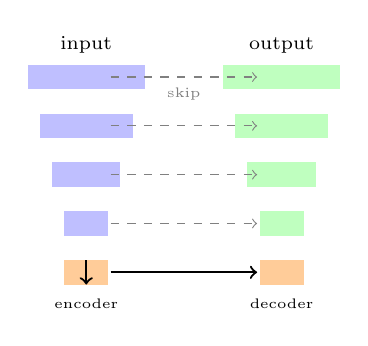
\begin{tikzpicture}[scale=0.62, every node/.style={font=\scriptsize}]
    \foreach \y/\w in {0/2.4, -1/1.9, -2/1.4, -3/0.9} {
      \fill[blue!25] (-\w/2,\y) rectangle (\w/2,\y+0.5);
      \fill[green!25] (4-\w/2,\y) rectangle (4+\w/2,\y+0.5);
    }
    \fill[orange!40] (-0.45,-4) rectangle (0.45,-3.5);
    \fill[orange!40] (3.55,-4) rectangle (4.45,-3.5);
    \node at (0,0.9) {input};
    \node at (4,0.9) {output};
    \draw[->,thick] (0,-3.5) -- (0,-4);
    \draw[->,thick] (0.5,-3.75) -- (3.5,-3.75);
    \foreach \y in {0,-1,-2,-3}
      \draw[->,dashed,gray] (0.5,\y+0.25) -- (3.5,\y+0.25);
    \node[gray] at (2,-0.1) {\tiny skip};
    \node at (0,-4.4) {\tiny encoder};
    \node at (4,-4.4) {\tiny decoder};
  \end{tikzpicture}
  \end{column}
  \end{columns}
\end{frame}

\begin{frame}[fragile]{\texttt{build\_unet}: the functional pattern}
\begin{columns}[T,onlytextwidth]
\begin{column}{0.42\textwidth}
\small
Built with the \textbf{Keras functional API}: each layer is \emph{called} on the previous tensor,
and the chain of calls defines the graph.\\[0.4em]
One encoder block = two convs then a pool. One decoder block = up-sample, a conv, then
\texttt{concatenate} with the saved encoder tensor (\texttt{conv3}), then two convs.\\[0.4em]
The pattern repeats symmetrically; only the channel counts change. The final $1\times1$ conv with
\texttt{softmax} produces the 4-class map.
\end{column}
\begin{column}{0.56\textwidth}
\begin{lstlisting}[firstnumber=last]
def build_unet(inputs, ker_init, dropout):
    # --- encoder block (x2 conv, then pool) ---
    c1 = Conv2D(32, 3, activation='relu',
                padding='same', kernel_initializer=ker_init)(inputs)
    c1 = Conv2D(32, 3, ...)(c1)
    p1 = MaxPooling2D((2, 2))(c1)
    # ... deeper blocks: 64, 128, 256 ...

    # --- bottleneck with dropout ---
    c5 = Conv2D(512, 3, ...)(p4)
    c5 = Conv2D(512, 3, ...)(c5)
    d5 = Dropout(dropout)(c5)

    # --- decoder block: upsample + skip-connect ---
    u7 = Conv2D(256, 2, ...)(UpSampling2D((2, 2))(d5))
    m7 = concatenate([c3, u7], axis=3)   # <- skip
    c7 = Conv2D(256, 3, ...)(m7)
    # ... mirror back up to 32 ...

    out = Conv2D(4, (1, 1), activation='softmax')(c9)
    return Model(inputs=inputs, outputs=out)
\end{lstlisting}
\end{column}
\end{columns}
\end{frame}

\begin{frame}[fragile]{Python syntax: the functional ``call'' chaining}
\begin{columns}[T,onlytextwidth]
\begin{column}{0.42\textwidth}
\small
\textbf{\texttt{Conv2D(...)(x)} -- two sets of parentheses.}\\[0.4em]
The first \texttt{Conv2D(32, 3, ...)} \emph{constructs} a layer object (with its weights and
settings).\\[0.4em]
The second \texttt{(x)} \emph{calls} that object on a tensor \texttt{x}, returning a new tensor.
Layers are callable, like functions.\\[0.4em]
By naming the outputs (\texttt{c1}, \texttt{c3}, \dots) we can reuse an earlier tensor later --
that is exactly how a \textbf{skip connection} is wired with \texttt{concatenate([c3, u7])}.
\end{column}
\begin{column}{0.56\textwidth}
\begin{lstlisting}[stepnumber=0]
# Step 1: construct a layer (an object)
layer = Conv2D(32, 3, activation='relu')

# Step 2: call it on a tensor -> new tensor
x = layer(inputs)

# Usually written in one line:
x = Conv2D(32, 3, activation='relu')(inputs)

# Saving a tensor to reuse it later (skip link):
c3 = Conv2D(256, 3, ...)(p2)
...
m7 = concatenate([c3, u7], axis=3)
\end{lstlisting}
\end{column}
\end{columns}
\end{frame}

% =====================================================================
\section{Training}

\begin{frame}[fragile]{Compile, callbacks, and fit}
\begin{columns}[T,onlytextwidth]
\begin{column}{0.42\textwidth}
\small
\texttt{compile} attaches the loss, the optimizer, and the long list of metrics we defined.\\[0.4em]
\textbf{Callbacks} run automatically during training:
\begin{itemize}
  \item \texttt{ReduceLROnPlateau} lowers the learning rate when \texttt{val\_loss} stalls,
  \item \texttt{ModelCheckpoint} saves the weights \emph{only when they improve},
  \item \texttt{CSVLogger} writes per-epoch metrics to a file.
\end{itemize}
\texttt{fit} then trains for 25 epochs, streaming batches from the generators.
\end{column}
\begin{column}{0.56\textwidth}
\begin{lstlisting}[firstnumber=last]
model.compile(
    loss="categorical_crossentropy",
    optimizer=keras.optimizers.Adam(learning_rate=1e-3),
    metrics=['accuracy', tf.keras.metrics.MeanIoU(4),
             dice_coef, precision, sensitivity, ...])

callbacks = [
    keras.callbacks.ReduceLROnPlateau(
        monitor='val_loss', factor=0.2, patience=2),
    keras.callbacks.ModelCheckpoint(
        'model_.{epoch:02d}-{val_loss:.6f}.weights.h5',
        save_best_only=True, save_weights_only=True),
    CSVLogger('training.log')]

history = model.fit(training_generator,
                    epochs=25,
                    steps_per_epoch=len(train_ids),
                    callbacks=callbacks,
                    validation_data=valid_generator)
\end{lstlisting}
\end{column}
\end{columns}
\end{frame}

\begin{frame}[fragile]{Saving and reloading the model}
\begin{columns}[T,onlytextwidth]
\begin{column}{0.42\textwidth}
\small
\texttt{model.save} writes the full model (architecture + weights) to one \texttt{.keras} file.\\[0.4em]
On reload, Keras does not know our \emph{custom} functions (\texttt{dice\_coef}, \texttt{precision},
\dots), so we pass them in \texttt{custom\_objects} -- a dictionary mapping the saved name back to
the Python function.\\[0.4em]
\texttt{compile=False} loads the graph without recompiling, which is enough for inference.
\end{column}
\begin{column}{0.56\textwidth}
\begin{lstlisting}[firstnumber=last]
model.save("my_model.keras")

model = keras.models.load_model(
    './my_model.keras',
    custom_objects={
        "accuracy": tf.keras.metrics.MeanIoU(num_classes=4),
        "dice_coef": dice_coef,
        "precision": precision,
        "sensitivity": sensitivity,
        "specificity": specificity,
        "dice_coef_necrotic": dice_coef_necrotic,
        "dice_coef_edema": dice_coef_edema,
        "dice_coef_enhancing": dice_coef_enhancing,
    },
    compile=False)
\end{lstlisting}
\end{column}
\end{columns}
\end{frame}

\begin{frame}[fragile]{Picking the best checkpoint automatically}
\begin{columns}[T,onlytextwidth]
\begin{column}{0.42\textwidth}
\small
Every checkpoint filename embeds its validation loss, e.g.\\
\texttt{model\_.19-0.026269.weights.h5}.\\[0.4em]
Rather than hard-coding one filename, we \texttt{glob} all of them and pick the one with the
\textbf{lowest} \texttt{val\_loss}.\\[0.4em]
\textbf{The \texttt{key=lambda} pattern:} \texttt{min} compares items by whatever the \texttt{key}
function returns. Here the lambda extracts the loss number out of the filename, so \texttt{min}
returns the best-performing checkpoint.
\end{column}
\begin{column}{0.56\textwidth}
\begin{lstlisting}[firstnumber=last]
checkpoints = glob.glob('model_.*.weights.h5')

best_checkpoint = min(
    checkpoints,
    key=lambda f: float(
        f.rsplit('-', 1)[1].replace('.weights.h5', '')))

print("Loading best checkpoint:", best_checkpoint)
best_saved_model.load_weights(best_checkpoint)
\end{lstlisting}
\vspace{0.4em}
\scriptsize \textbf{How the lambda parses the name:}\\
\texttt{"model\_.19-0.026269.weights.h5"}\\
$\xrightarrow{\text{rsplit('-',1)[1]}}$ \texttt{"0.026269.weights.h5"}\\
$\xrightarrow{\text{replace(...)}}$ \texttt{"0.026269"}
$\xrightarrow{\text{float}}$ \texttt{0.026269}
\end{column}
\end{columns}
\end{frame}

% =====================================================================
\section{Prediction and evaluation}

\begin{frame}[fragile]{Predicting a patient's segmentation}
\begin{columns}[T,onlytextwidth]
\begin{column}{0.42\textwidth}
\small
Inference mirrors the generator: load FLAIR + T1ce, resize 100 slices to $128\times128$, stack into
the two-channel input, and call \texttt{model.predict}.\\[0.4em]
The output \texttt{p} has shape $(100, 128, 128, 4)$ -- a probability per class for every pixel of
every slice. Channels 1/2/3 are core / edema / enhancing.\\[0.4em]
Note both the prediction and the visualization helpers build their paths through the same
\texttt{imgPath} helper from the start of the deck.
\end{column}
\begin{column}{0.56\textwidth}
\begin{lstlisting}[firstnumber=last]
def predictByPath(case):
    X = np.empty((VOLUME_SLICES, IMG_SIZE, IMG_SIZE, 2))
    flair = nib.load(imgPath(case, 'flair')).get_fdata()
    ce    = nib.load(imgPath(case, 't1ce')).get_fdata()
    for j in range(VOLUME_SLICES):
        X[j,:,:,0] = cv2.resize(
            flair[:,:,j+VOLUME_START_AT], (IMG_SIZE,)*2)
        X[j,:,:,1] = cv2.resize(
            ce[:,:,j+VOLUME_START_AT], (IMG_SIZE,)*2)
    return model.predict(X / np.max(X), verbose=1)

# p[:, :, :, 1] -> core
# p[:, :, :, 2] -> edema
# p[:, :, :, 3] -> enhancing
\end{lstlisting}
\end{column}
\end{columns}
\end{frame}

\begin{frame}[fragile]{Final evaluation on the test set}
\begin{columns}[T,onlytextwidth]
\begin{column}{0.42\textwidth}
\small
\texttt{model.evaluate} runs the test generator and returns the loss plus every metric, in the same
order they were listed at \texttt{compile} time.\\[0.4em]
\textbf{\texttt{zip}} pairs each number with its human-readable description; iterating the zip prints a
tidy report.\\[0.4em]
The metrics that matter most here are the \textbf{per-class Dice} scores -- they tell us how well
each tumor region is segmented, not just overall pixel accuracy.
\end{column}
\begin{column}{0.56\textwidth}
\begin{lstlisting}[firstnumber=last]
results = model.evaluate(test_generator,
                         batch_size=100,
                         callbacks=callbacks)

descriptions = ["Loss", "Accuracy", "MeanIOU",
    "Dice coefficient", "Precision", "Sensitivity",
    "Specificity", "Dice Necrotic", "Dice Edema",
    "Dice Enhancing"]

for metric, desc in zip(results, descriptions):
    print(f"{desc} : {round(metric, 4)}")
\end{lstlisting}
\end{column}
\end{columns}
\end{frame}

% =====================================================================
\section{Conclusion}

\begin{frame}{What we covered}
  \begin{itemize}
    \item Reading \texttt{.nii} MRI volumes and scaling them for the network.
    \item Centralizing file-path logic in a single \texttt{imgPath} helper.
    \item Streaming data efficiently with a \texttt{keras.utils.Sequence} generator.
    \item The Dice coefficient and why it beats accuracy for tumor segmentation.
    \item The U-Net encoder--decoder with skip connections, built via the functional API.
    \item Training with callbacks, and selecting the best checkpoint automatically.
    \item Predicting and visualizing tumor sub-regions on unseen patients.
  \end{itemize}
  \vspace{0.5em}
  The notebook is a compact, end-to-end example of medical image segmentation -- from raw scans to a
  trained model and per-class evaluation.
\end{frame}

\begin{frame}[standout]
  Questions?
\end{frame}

\end{document}
